%%% main.tex — 习题册控制器 %%%
%%% 编译：latexmk -xelatex main.tex %%%

\documentclass[12pt,a4paper,oneside]{ctexbook}

%%% 页面布局（习题册：左窄右宽，留给右栏答题区）%%%
\usepackage[left=1.5cm, right=1.5cm, top=2.5cm, bottom=2.5cm, headheight=25pt]{geometry}

%%% 导言区模块 %%%
%%% packages.tex — 宏包调用 %%%

%%% 页面布局 %%%
% geometry 在各主文件中单独配置（习题册和答案册页边距不同）

%%% 基础数学包 %%%
\usepackage{amsmath}
\usepackage{amssymb}
\usepackage{amsthm}

%%% 超链接 %%%
\usepackage[colorlinks=true, linkcolor=black, citecolor=black]{hyperref}

%%% 数学字体 %%%
\usepackage{unicode-math}
\setmathfont{NewCMMath-Regular.otf}

%%% 绘图 %%%
\usepackage{tikz}
\usetikzlibrary{positioning, calc, shapes.geometric, decorations.pathreplacing}

%%% 选择题选项 %%%
\usepackage{tasks}
\settasks{
	label = \Alph*.,
	label-width = 1.8em,
	item-indent = 2.3em,
	label-offset = 0.5em,
	column-sep=1.5em
}

%%% 高级文档命令 %%%
\usepackage{xparse}

%%% 彩色方框 %%%
\usepackage[most]{tcolorbox}
\tcbuselibrary{skins, breakable}

%%% 习题与解析管理 %%%
\usepackage{xsim}

%%% 页眉页脚 %%%
\usepackage{fancyhdr}

%%% colors.tex — 颜色定义 %%%

%%% 灰度颜色方案（封面/封底除外）%%%
\definecolor{maincolor}{gray}{0.25}          % 深灰
\definecolor{accentcolor}{gray}{0.45}        % 中灰
\definecolor{lightbg}{gray}{0.96}            % 极浅灰底
\definecolor{notecolor}{gray}{0.40}          % 注释框边灰
\definecolor{notebg}{gray}{0.97}             % 注释框底灰
\definecolor{kpcolor}{gray}{0.35}            % 考点图标灰
\definecolor{rulegray}{gray}{0.50}           % 竖线颜色
\definecolor{answercolor}{gray}{0.85}         % 答题区底色

%%% 封面/封底专用橙色系 %%%
\definecolor{coverorange}{RGB}{230, 105, 25}     % Springer 橙
\definecolor{coverdark}{RGB}{50, 50, 55}          % 深炭灰
\definecolor{coverlight}{RGB}{255, 243, 228}      % 暖奶白
\definecolor{coveramber}{RGB}{180, 80, 15}        % 深琥珀

%%% fonts.tex — 字体配置 %%%

%%% CJK 字体 %%%
\setCJKmainfont{SimSun}[BoldFont=SimHei, ItalicFont=STKaiti]
\setCJKsansfont{SimHei}
\setCJKmonofont{FangSong}

%%% 数学字体 %%%
% \setmathfont 已在 packages.tex 中通过 unicode-math 设置

%%% macros.tex — 语义化命令与工具宏 %%%

%%% 语义化数学符号 %%%
\newcommand{\dd}{\mathrm{d}}           % 微分符号 d
\newcommand{\ee}{\mathrm{e}}           % 自然常数 e
\newcommand{\ii}{\mathrm{i}}           % 虚数单位 i
\newcommand{\R}{\mathbb{R}}            % 实数集
\newcommand{\N}{\mathbb{N}}            % 自然数集
\newcommand{\Z}{\mathbb{Z}}            % 整数集
\newcommand{\Q}{\mathbb{Q}}            % 有理数集

%%% 考点菱形图标 %%%
\newcommand{\knowledgepointicon}{%
	\tikz[baseline=-0.1ex] \node[
	fill=kpcolor,
	shape=diamond,
	aspect=0.7,
	inner sep=1.5pt
	] {};}

%%% 双栏答题区命令（习题册专用）%%%
% 这些命令仅在加载了 paracol 包时才有意义
% 答案册不加载 paracol，因此用 \providecommand 提供空定义

\providecommand{\answerdivider}{%
	\begin{tikzpicture}[overlay, remember picture]
		\draw[rulegray, line width=0.6pt]
			([xshift=-3pt]current page.north west |- 0,0) -- ++(0,-\textheight);
	\end{tikzpicture}%
}

\providecommand{\startexercise}{%
	\columnratio{0.58,0.42}%
	\columnsep=12pt%
	\begin{paracol}{2}%
}

\providecommand{\stopexercise}{%
	\end{paracol}%
}

%%% environments.tex — 习题环境定义（xsim + tcolorbox）%%%

%%% ==================== xsim 全局配置 ==================== %%%

\xsimsetup{
	exercise/name = 习题,
	solution/name = 解析,
}

%%% 自定义属性 %%%
\DeclareExerciseProperty{source}    % 题目来源
\DeclareExerciseProperty{topic}     % 知识点标签
\DeclareExerciseProperty{score}     % 分值

%%% ==================== 选择题类型（choice）==================== %%%

\DeclareExerciseType{choice}{
	exercise-env  = choice ,
	solution-env  = choice-sol ,
	exercise-name = 习题 ,
	solution-name = 解析 ,
	exercise-template = choice-default ,
	solution-template = solution-default ,
}

%%% 选择题 — 习题册模板（左栏题目 + 右栏答题卡）%%%
\DeclareExerciseEnvironmentTemplate{choice-default}{%
	\par\addvspace{\medskipamount}%
	\begin{tcolorbox}[
		enhanced,
		breakable,
		colback=lightbg,
		colframe=maincolor,
		boxrule=0.4pt,
		arc=2pt,
		left=5mm,
		right=3mm,
		top=4pt,
		bottom=4pt,
		boxsep=0pt,
		before upper={
			\noindent
			\textbf{\color{maincolor}\GetExerciseName\ \GetExerciseProperty{counter}}
			\hfill
			\IfExercisePropertySetTF{topic}{\knowledgepointicon~\GetExerciseProperty{topic}}{}
			\IfExercisePropertySetT{source}{\quad{\color{accentcolor}[\ \textbf{\GetExerciseProperty{source}}\ ]}}
			\par\vspace{1ex}
		}
	]
}{%
	\end{tcolorbox}%
	% 习题册模式（非打印解析时）：切换到右栏绘制答题卡
	\IfSolutionPrintF{%
		\switchcolumn%
		\vspace{\medskipamount}%
		\begin{tcolorbox}[
			enhanced,
			colback=answercolor,
			colframe=rulegray,
			boxrule=0.3pt,
			arc=1pt,
			left=4mm,
			right=3mm,
			top=4pt,
			bottom=4pt,
			boxsep=0pt,
			before upper={
				\noindent\textbf{\scriptsize\color{maincolor}答 \GetExerciseProperty{counter}}\par\vspace{2pt}
				\scriptsize
			}
		]%
		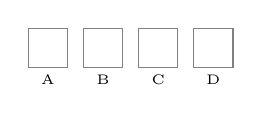
\begin{tikzpicture}[
			optbox/.style={rectangle, draw=rulegray, minimum size=5mm, inner sep=0pt},
		]
			\foreach \l [count=\c] in {A,B,C,D} {
				\node[optbox] at (\c*7mm, 0) {};
				\node[font=\tiny] at (\c*7mm, -4mm) {\l};
			}
		\end{tikzpicture}%
		\end{tcolorbox}%
		\switchcolumn*%
	}%
}

%%% 选择题 — 答案册模板（仅解析）%%%
% choice-sol 使用下方的 solution-default 通用模板

%%% ==================== 解答题类型（prob）==================== %%%
% 注：命名为 prob 而非 exercise，以避免与 xsim 内置 exercise 类型冲突

\DeclareExerciseType{prob}{
	exercise-env  = prob ,
	solution-env  = prob-sol ,
	exercise-name = 习题 ,
	solution-name = 解析 ,
	exercise-template = prob-default ,
	solution-template = solution-default ,
}

%%% 解答题 — 习题册模板（左栏题目 + 右栏作答横线）%%%
\DeclareExerciseEnvironmentTemplate{prob-default}{%
	\par\addvspace{\medskipamount}%
	\begin{tcolorbox}[
		enhanced,
		breakable,
		colback=lightbg,
		colframe=maincolor,
		boxrule=0.4pt,
		arc=2pt,
		left=5mm,
		right=3mm,
		top=4pt,
		bottom=4pt,
		boxsep=0pt,
		before upper={
			\noindent
			\textbf{\color{maincolor}\GetExerciseName\ \GetExerciseProperty{counter}}
			\IfExercisePropertySetT{source}{\ {\color{accentcolor}\GetExerciseProperty{source}}}
			\IfExercisePropertySetT{score}{\quad{\color{accentcolor}[本题 \GetExerciseProperty{score} 分]}}
			\hfill
			\IfExercisePropertySetTF{topic}{\knowledgepointicon~\GetExerciseProperty{topic}}{}
			\par\vspace{1ex}
		}
	]
}{%
	\end{tcolorbox}%
	% 习题册模式（非打印解析时）：切换到右栏绘制作答区
	\IfSolutionPrintF{%
		\switchcolumn%
		\vspace{\medskipamount}%
		\begin{tcolorbox}[
			enhanced,
			colback=answercolor,
			colframe=rulegray,
			boxrule=0.3pt,
			arc=1pt,
			left=4mm,
			right=3mm,
			top=4pt,
			bottom=4pt,
			boxsep=0pt,
			before upper={
				\noindent\textbf{\scriptsize\color{maincolor}答 \GetExerciseProperty{counter}}\par\vspace{2pt}
				\scriptsize
			}
		]%
		\color{rulegray}%
		\foreach \i in {1,...,3}{%
			\rule{\linewidth}{0.3pt}\par\vspace{8mm}%
		}%
		\end{tcolorbox}%
		\switchcolumn*%
	}%
}

%%% 解答题 — 答案册模板（仅解析）%%%
% prob-sol 使用下方的 solution-default 通用模板

%%% ==================== 通用解析模板 ==================== %%%

\DeclareExerciseEnvironmentTemplate{solution-default}{%
	\par\addvspace{\medskipamount}%
	\begin{tcolorbox}[
		enhanced, breakable,
		colback=lightbg,
		colframe=maincolor,
		boxrule=0.4pt,
		arc=2pt,
		left=5mm,
		right=3mm,
		top=4pt,
		bottom=4pt,
		boxsep=0pt,
		before upper={
			\noindent
			\textbf{\color{maincolor}\GetExerciseName\ \GetExerciseProperty{counter}}
			\IfExercisePropertySetT{topic}{\hfill\knowledgepointicon~\GetExerciseProperty{topic}}
			\par\vspace{0.5ex}
		}
	]
}{%
	\end{tcolorbox}%
}

%%% ==================== 辅助环境 ==================== %%%

%%% 注释环境 %%%
\newtcolorbox{note}[1][]{%
	enhanced, breakable,
	colback=notebg,
	colframe=notecolor,
	boxrule=0.4pt,
	arc=2pt,
	left=5mm,
	right=3mm,
	top=4pt,
	bottom=4pt,
	boxsep=0pt,
	before upper={
		\noindent\textbf{\color{notecolor}注}\par\vspace{0.5ex}
	},
	#1
}

%%% 知识框架环境 %%%
\newtcolorbox{knowledgeframe}{%
	enhanced, breakable,
	colback=lightbg,
	colframe=maincolor,
	boxrule=0.4pt,
	arc=2pt,
	left=5mm,
	right=3mm,
	top=4pt,
	bottom=4pt,
	boxsep=0pt,
	before upper={
		\noindent
		\textbf{\color{maincolor}知识框架}
		\hfill
		\knowledgepointicon~\text{要点回顾}
		\par\vspace{1ex}
	}
}


%%% 习题册专有：双栏答题区 %%%
\usepackage{paracol}

%%% 页眉页脚 %%%
\newcommand{\booktitle}{高中数学之旅（习题集）}
%%% pagestyle.tex — 页眉页脚配置 %%%
% 使用前需定义 \exercisetitle 或 \solutionstitle 命令
% 分别在 main.tex 和 main_solutions.tex 中设置

\pagestyle{fancy}
\fancyhf{}
\fancyhead[L]{\small\color{maincolor}\booktitle}
\fancyhead[R]{\small\color{maincolor}\leftmark}
\fancyfoot[C]{\thepage}
\renewcommand{\headrulewidth}{0.4pt}
\renewcommand{\headrule}{\hbox to\headwidth{\color{maincolor}\leaders\hrule height\headrulewidth\hfill}}


\begin{document}

%%% 封面 %%%
\input{covers/cover-exercise}

\pagenumbering{roman}
\frontmatter
\pagestyle{plain}
\tableofcontents

\mainmatter
\pagestyle{fancy}

%%% 各章内容 %%%
\chapter{集合和逻辑用语}

%% ---- 知识框架 ---- %%
\begin{knowledgeframe}
\begin{itemize}
	\item \textbf{集合的基本概念}：元素与集合的关系（$\in, \notin$）、集合的表示法（列举法、描述法）、常用数集符号（$\N, \Z, \Q, \R$）。
	\item \textbf{集合间的关系}：子集（$\subseteq$）、真子集（$\subsetneq$）、相等（$=$）、空集（$\emptyset$）。
	\item \textbf{集合的基本运算}：交集（$\cap$）、并集（$\cup$）、补集（$\complement_U A$）、差集（$A \setminus B$）。
	\item \textbf{运算律}：德摩根定律——$\complement_U(A \cup B) = (\complement_U A) \cap (\complement_U B)$，\ $\complement_U(A \cap B) = (\complement_U A) \cup (\complement_U B)$。
	\item \textbf{容斥原理}：$|A \cup B| = |A| + |B| - |A \cap B|$，\ 三集合推广公式。
	\item \textbf{逻辑用语}：充分条件与必要条件（$p \Rightarrow q$）、全称量词与存在量词及其否定、命题的四种形式。
\end{itemize}
\end{knowledgeframe}

%% ---- 第一节：集合的基本运算 ---- %%
\section{集合的基本运算}

\startexercise

\subsection*{A组}

\begin{choice}[topic={量词命题的否定}]
已知命题 $p: \exists x \in \mathbb{N}, x^2 \le 0$，则 $\neg p$ 为
\begin{tasks}(2)
	\task $\exists x \in \mathbb{N}, x^2 \le 0$
	\task $\exists x \in \mathbb{N}, x^2 > 0$
	\task $\forall x \in \mathbb{N}, x^2 > 0$
	\task $\forall x \in \mathbb{N}, x^2 \ge 0$
\end{tasks}
\end{choice}
\begin{choice-sol}
\textbf{答案 C}

本题考查全称量词命题与存在量词命题的否定关系.
否定一个量词命题，遵循"改量词，否结论"的原则.
原命题 $p$ 为一个存在量词命题，其逻辑形式为 $\exists x \in M, P(x)$.

其否定的一般形式为：
\[ \neg (\exists x \in M, P(x)) \iff \forall x \in M, \neg P(x) \]
在本题中，量词 $\exists$ (存在) 的否定是 $\forall$ (任意).
原结论 $P(x)$ 为 $x^2 \le 0$，其否定 $\neg P(x)$ 为 $x^2 > 0$.

故 $\neg p$ 为 $\forall x \in \mathbb{N}, x^2 > 0$。

\begin{note}
选项 D 中，$x^2 \ge 0$ 在自然数范围内是恒成立的，
但它并非 $x^2 \le 0$ 的严格否定.
一个结论的否定是其逻辑补集，而非简单的反义关系.
对于实数 $y$，$y \le 0$ 的否定是 $y>0$。
\end{note}
\end{choice-sol}

\begin{choice}[source={2023 秋 · 高一 · 重庆永川区 · 月考校考}, topic={集合的补集与交集}]
设集合 $A=\{x\mid x<2 \text{或} x \ge 4\}$, $B=\{x\mid x<a\}$，若 $(\complement_U A) \cap B \neq \emptyset$，则 $a$ 的取值范围是
\begin{tasks}(2)
	\task $a < 2$
	\task $a > 2$
	\task $a \le 4$
	\task $a \ge 4$
\end{tasks}
\end{choice}
\begin{choice-sol}
\textbf{答案 B}

本题的核心思想是将抽象的集合运算转化为直观的数轴位置关系.
首先，根据集合 $A$ 的定义，确定其在全集 $U=\mathbb{R}$ 下的补集。
\[ A = \{x\mid x<2 \text{ 或 } x \ge 4\} = (-\infty, 2) \cup [4, +\infty) \]
其补集为数轴上未被覆盖的部分：
\[ \complement_U A = \{x\mid 2 \le x < 4\} = [2, 4) \]
集合 $B$ 的定义为：
\[ B = \{x\mid x<a\} = (-\infty, a) \]
题目条件为 $(\complement_U A) \cap B \neq \emptyset$，
即区间 $[2, 4)$ 与 $(-\infty, a)$ 的交集不为空.
为满足此条件，区间 $(-\infty, a)$ 的右端点 $a$
必须大于区间 $[2,4)$ 的左端点 $2$.
因此，可得 $a > 2$。
\end{choice-sol}

\begin{choice}[topic={集合的交集与子集个数}]
已知集合 $A=\{(x,y) \mid x,y \in \mathbb{Z}, \text{且 } xy=4\}$, $B=\{(x,y) \mid x \le y\}$，则 $A \cap B$ 的子集的个数为
\begin{tasks}(4)
	\task 3
	\task 4
	\task 8
	\task 16
\end{tasks}
\end{choice}
\begin{choice-sol}
\textbf{答案 D}

解题分为两个步骤：首先确定交集 $A \cap B$ 的所有元素，然后利用子集个数公式求解.

第一步，列举集合 $A$ 的所有元素.
$A$ 的元素是满足 $xy=4$ 的整数坐标点 $(x,y)$。
\[ A = \{(1,4), (4,1), (-1,-4), (-4,-1), (2,2), (-2,-2)\} \]
第二步，从 $A$ 中筛选出满足集合 $B$ 条件 ($x \le y$) 的元素.
\[ A \cap B = \{(1,4), (-4,-1), (2,2), (-2,-2)\} \]
集合 $A \cap B$ 中含有 4 个元素.

一个含有 $n$ 个元素的有限集合，其子集的个数为 $2^n$.
本题中 $n=4$，故子集个数为 $2^4 = 16$。
\end{choice-sol}


\subsection*{B组}

\begin{choice}[source={2023 秋 · 高一 · 山东烟台 · 月考校考}, topic={充分必要条件}]
下列说法错误的是
\begin{tasks}(1)
	\task ``$A \cap B = B$'' 是 ``$B = \emptyset$'' 的必要不充分条件
	\task ``$x=3$'' 的一个充分不必要条件是 ``$x^2-2x-3=0$''
	\task ``$\lvert x\rvert=1$'' 是 ``$x=1$'' 的必要不充分条件
	\task ``$m$ 是实数'' 的一个充分不必要条件是 ``$m$ 是有理数''
\end{tasks}
\end{choice}
\begin{choice-sol}
\textbf{答案 D}

本题考查充分条件与必要条件的判断.
核心方法是将命题间的逻辑关系转化为集合间的包含关系：
若 $p \Rightarrow q$，则 $p$ 对应的集合是 $q$ 对应集合的子集.

A. ``$A \cap B = B$'' 等价于 $B \subseteq A$.
``$B=\emptyset$'' 能够推出 $B \subseteq A$，但反之不成立.
因此，``$B \subseteq A$'' 是 ``$B=\emptyset$'' 的必要不充分条件.该说法正确.

B. ``$x=3$'' 对应集合 $\{3\}$.
``$x^2-2x-3=0$'' 对应解集 $\{3, -1\}$.
因为 $\{3\} \subsetneq \{3, -1\}$，
所以前者是后者的充分不必要条件.该说法正确.

C. ``$\lvert x\rvert=1$'' 对应集合 $\{1, -1\}$.
``$x=1$'' 对应集合 $\{1\}$.
因为 $\{1\} \subsetneq \{1, -1\}$，
所以前者是后者的必要不充分条件.该说法正确.

D. 命题 $p$: ``$m$ 是有理数''，对应集合 $\mathbb{Q}$.
命题 $q$: ``$m$ 是实数''，对应集合 $\mathbb{R}$.
因为 $\mathbb{Q} \subsetneq \mathbb{R}$，
所以 $p$ 是 $q$ 的充分不必要条件.
原说法颠倒了主次，故错误.
\end{choice-sol}

\begin{choice}[topic={全称命题的否定}]
若命题 ``$\forall x \in \mathbb{R}, 1-x^2 \le m$'' 是假命题，则实数 $m$ 的取值范围是
\begin{tasks}(2)
	\task $(-\infty, 1)$
	\task $(-\infty, 1]$
	\task $(1, +\infty)$
	\task $[1, +\infty)$
\end{tasks}
\end{choice}
\begin{choice-sol}
\textbf{答案 A}

一个全称量词命题为假，其逻辑等价于它的否定形式（一个存在量词命题）为真.
设原命题为 $P: \forall x \in \mathbb{R}, 1-x^2 \le m$。

由于命题 $P$ 为假，其否定命题 $\neg P$ 必为真.
\[ \neg P: \exists x \in \mathbb{R}, \neg(1-x^2 \le m) \implies \exists x \in \mathbb{R}, 1-x^2 > m \]
该存在量词命题为真，意味着 $m$ 必须小于函数 $f(x) = 1-x^2$ 的最大值.
函数 $f(x)=1-x^2$ 是一个开口向下的二次函数，其顶点为最大值点.
\[ f(x)_{\max} = f(0) = 1 \]
因此，实数 $m$ 的取值范围必须是 $m < 1$，
即 $m \in (-\infty, 1)$。
\end{choice-sol}

\begin{choice}[topic={充分不必要条件的应用}]
若 ``$x=2$'' 是 ``$m^2x^2 - (m+3)x + 4 = 0$'' 的充分不必要条件，则实数 $m$ 的值为
\begin{tasks}(2)
	\task 1
	\task $-\frac{1}{2}$
	\task $-\frac{1}{2}$ 或 1
	\task -1 或 $-\frac{1}{2}$
\end{tasks}
\end{choice}
\begin{choice-sol}
\textbf{答案 B}

命题``$p$ 是 $q$ 的充分不必要条件''包含两层含义，必须同时满足：
\begin{itemize}
	\item \textbf{充分性}: $p \Rightarrow q$。
	\item \textbf{不必要性}: $q \not\Rightarrow p$。
\end{itemize}
设 $p: x=2$，$q: m^2x^2 - (m+3)x + 4 = 0$。

\textbf{检验充分性}:
将 $x=2$ 代入方程 $q$ 中，方程必须成立.
\[ 4m^2 - 2(m+3) + 4 = 0 \implies 2m^2 - m - 1 = 0 \]
因式分解得 $(2m+1)(m-1) = 0$，
解得 $m=1$ 或 $m=-\frac{1}{2}$。

\textbf{检验不必要性}:
方程 $q$ 的解集 $S$ 必须真包含 $\{2\}$，即 $S \neq \{2\}$。
\begin{itemize}
	\item 当 $m=1$ 时，方程为 $x^2 - 4x + 4 = 0$，
	解集 $S=\{2\}$.
	此时 $q \Rightarrow p$ 成立，不满足``不必要''条件，故舍去.
	\item 当 $m=-\frac{1}{2}$ 时，
	方程为 $\frac{1}{4}x^2 - \frac{5}{2}x + 4 = 0$，
	即 $x^2 - 10x + 16 = 0$.
	解集 $S=\{2, 8\}$.
	此时 $S \neq \{2\}$，满足``不必要''条件。
\end{itemize}
综上，唯一满足条件的实数 $m$ 的值为 $-\frac{1}{2}$。
\end{choice-sol}

\begin{choice}[topic={集合的补集与互异性}]
设全集 $U=\{1,2,3,4,5\}$，集合 $A=\{1,a,b\}, B=\{4, a-b\}$.若 $\complement_U A = B$，则 $a,b$ 的值分别为
\begin{tasks}(2)
	\task 3,2
	\task 4,3
	\task 3,2 或 5,3
	\task 5,2 或 5,3
\end{tasks}
\end{choice}
\begin{choice-sol}
\textbf{答案 D}

条件 $\complement_U A = B$ 是解题的关键，
它等价于以下两个条件同时成立：
\[ A \cup B = U \quad \text{且} \quad A \cap B = \emptyset \]
根据题意：
$U=\{1,2,3,4,5\}$
$A=\{1,a,b\}$
$B=\{4, a-b\}$

由 $A \cup B = U$，可得：
\[ \{1,a,b\} \cup \{4, a-b\} = \{1, a, b, 4, a-b\} = \{1,2,3,4,5\} \]
比较两集合，可知无序集合 $\{a, b, a-b\}$ 必须与 $\{2,3,5\}$ 相等.
同时，集合 A 和 B 的元素必须满足互异性.

我们通过分类讨论来寻找 $a,b$ 的取值：
\begin{itemize}
	\item \textbf{情况一：} 设 $a=5, b=2$.
	则 $a-b = 3$.
	此时 $\{a,b,a-b\} = \{5,2,3\}$ 与 $\{2,3,5\}$ 匹配.
	检验：$A=\{1,5,2\}, B=\{4,3\}$.
	此时 $\complement_U A = \{3,4\}=B$，符合题意.
	\item \textbf{情况二：} 设 $a=5, b=3$.
	则 $a-b = 2$.
	此时 $\{a,b,a-b\} = \{5,3,2\}$ 与 $\{2,3,5\}$ 匹配.
	检验：$A=\{1,5,3\}, B=\{4,2\}$.
	此时 $\complement_U A = \{2,4\}=B$，符合题意。
\end{itemize}
其他组合（如 $a=3,b=2$ 时 $a-b=1$,与$A$中元素重复）均不满足条件.
因此，$a,b$ 的值为 5,2 或 5,3。
\end{choice-sol}


\subsection*{C组}

\begin{choice}[source={2024 秋 · 高一 · 福建龙岩 · 开学考试校考}, topic={新定义集合与元素互异性}]
定义集合 $A \otimes B = \{x \mid x=\sqrt{a^2+b^2}, a \in A, b \in B\}$，若 $A=\{n, -1\}, B=\{\sqrt{2}, 1\}$，且集合 $A \otimes B$ 中有 3 个元素，则由实数 $n$ 的所有取值组成的集合的非空真子集的个数为
\begin{tasks}(4)
	\task 2
	\task 6
	\task 14
	\task 15
\end{tasks}
\end{choice}
\begin{choice-sol}
\textbf{答案 B}

本题综合考查了新定义集合的理解、集合元素的互异性以及子集个数的计算.

\textbf{1. 构造集合 $A \otimes B$}
根据定义，$A=\{n, -1\}, B=\{\sqrt{2}, 1\}$。
\[ A \otimes B = \{\sqrt{n^2 + (\sqrt{2})^2}, \sqrt{n^2 + 1^2}, \sqrt{(-1)^2 + (\sqrt{2})^2}, \sqrt{(-1)^2 + 1^2}\} \]
化简得：
\[ A \otimes B = \{\sqrt{n^2+2}, \sqrt{n^2+1}, \sqrt{3}, \sqrt{2}\} \]

\textbf{2. 应用元素个数条件}
已知 $\lvert A \otimes B\rvert = 3$.
由于上式给出了 4 个表达式，根据集合元素的互异性，
其中必有两个表达式的值相等.
注意到 $\sqrt{n^2+2} > \sqrt{n^2+1}$ 且 $\sqrt{3} > \sqrt{2}$，
因此相等的只可能是一个含 $n$ 的项与一个常数项.

分类讨论：
\begin{itemize}
	\item 若 $\sqrt{n^2+1} = \sqrt{2} \implies n^2=1 \implies n=\pm 1$.
	此时 $\sqrt{n^2+2}=\sqrt{3}$，
	集合为 $\{\sqrt{2}, \sqrt{3}\}$，
	仅有 2 个元素，不合题意.
	\item 若 $\sqrt{n^2+1} = \sqrt{3} \implies n^2=2 \implies n=\pm \sqrt{2}$.
	此时 $\sqrt{n^2+2}=\sqrt{4}=2$，
	集合为 $\{2, \sqrt{3}, \sqrt{2}\}$，
	有 3 个元素，符合题意.
	\item 若 $\sqrt{n^2+2} = \sqrt{2} \implies n^2=0 \implies n=0$.
	此时 $\sqrt{n^2+1}=1$，
	集合为 $\{1, \sqrt{3}, \sqrt{2}\}$，
	有 3 个元素，符合题意.
	\item 若 $\sqrt{n^2+2} = \sqrt{3} \implies n^2=1$，
	情况同第一类，不符。
\end{itemize}

\textbf{3. 计算子集个数}
由上可知，实数 $n$ 的所有取值组成的集合为
$S_n = \{-\sqrt{2}, 0, \sqrt{2}\}$。
该集合有 $k=3$ 个元素.
非空真子集的个数为 $2^k - 2 = 2^3 - 2 = 6$。
\end{choice-sol}


\stopexercise

%% ---- 第二节：德摩根定律与容斥原理 ---- %%
\section{德摩根定律与容斥原理}

\startexercise

\subsection*{A组}

\begin{prob}[topic={集合的并集与补集运算}, score=5]
\textbf{(填空题)} 已知全集 $U=\{x \in \mathbb{Z} \mid -3 \le x \le 3\}$, 集合 $A=\{-2, 1, 2\}$, $B=\{-1, 0, 1\}$. 求 $\complement_U(A \cup B) = $ \rule{3cm}{0.5pt}.
\end{prob}
\begin{prob-sol}
\textbf{答案} $\{-3, 3\}$

本题考查有限集合的补集运算.

\textbf{方法一：直接法}
首先确定全集 $U$ 和并集 $A \cup B$。
\[ U = \{-3, -2, -1, 0, 1, 2, 3\} \]
\[ A \cup B = \{-2, 1, 2\} \cup \{-1, 0, 1\} = \{-2, -1, 0, 1, 2\} \]
$\complement_U(A \cup B)$ 即为在 $U$ 中但不在 $A \cup B$ 中的元素所构成的集合.
\[ \complement_U(A \cup B) = \{-3, 3\} \]

\textbf{方法二：德摩根定律}
根据德摩根定律，$\complement_U(A \cup B) = (\complement_U A) \cap (\complement_U B)$。
\[ \complement_U A = \{-3, -1, 0, 3\} \]
\[ \complement_U B = \{-3, -2, 2, 3\} \]
两补集的交集为：
\[ (\complement_U A) \cap (\complement_U B) = \{-3, 3\} \]
\end{prob-sol}

\begin{prob}[topic={容斥原理初步应用}, score=10]
\textbf{(解答题)} 某班有50名学生，参加数学兴趣小组的有25人，参加物理兴趣小组的有22人，两个小组都参加的有10人.问：
\begin{enumerate}
	\item 至少参加一个兴趣小组的学生有多少人？
	\item 两个小组都没有参加的学生有多少人？
\end{enumerate}
\end{prob}
\begin{prob-sol}
本题是容斥原理的直接应用.
设参加数学兴趣小组的学生集合为 $M$，
参加物理兴趣小组的学生集合为 $P$。
根据题意，已知信息为：
\[ \lvert M\rvert = 25, \quad \lvert P\rvert = 22, \quad \lvert M \cap P\rvert = 10 \]
(1) \textbf{至少参加一个兴趣小组的人数}，即求 $\lvert M \cup P\rvert$。
根据容斥原理公式：
\[ \lvert M \cup P\rvert = \lvert M\rvert + \lvert P\rvert - \lvert M \cap P\rvert = 25 + 22 - 10 = 37 \text{ (人)} \]

(2) \textbf{两个小组都没有参加的人数}.
设全班学生为全集 $U$，则所求人数为 $\lvert\complement_U(M \cup P)\rvert$。
\[ \lvert\complement_U(M \cup P)\rvert = \lvert U\rvert - \lvert M \cup P\rvert = 50 - 37 = 13 \text{ (人)} \]
\end{prob-sol}


\subsection*{B组}

\begin{prob}[topic={德摩根定律与一元二次不等式}, score=12]
\textbf{(解答题)} 设全集 $U=\mathbb{R}$, 集合 $A=\{x\mid x \le -1 \text{ 或 } x \ge 4\}$, $B=\{x\mid x^2-3x-4<0\}$.
\begin{enumerate}
	\item 求集合 $B$；
	\item 利用德摩根定律，求 $\complement_U(A \cap B)$.
\end{enumerate}
\end{prob}
\begin{prob-sol}
本题将德摩根定律与一元二次不等式的求解相结合.

(1) \textbf{求集合 B}
解不等式 $x^2-3x-4<0$。
因式分解得 $(x-4)(x+1)<0$，解得 $-1 < x < 4$。
\[ B=\{x \mid -1 < x < 4\} = (-1, 4) \]

(2) \textbf{求 $\complement_U(A \cap B)$}
直接计算 $A \cap B$ 再求补集较为繁琐，应用德摩根定律可以简化运算。
\[ \complement_U(A \cap B) = (\complement_U A) \cup (\complement_U B) \]
分别计算两个补集：
\[ \complement_U A = \{x \mid \neg(x \le -1 \text{ 或 } x \ge 4)\} = \{x \mid -1 < x < 4\} = (-1, 4) \]
\[ \complement_U B = \{x \mid \neg(-1 < x < 4)\} = \{x \mid x \le -1 \text{ 或 } x \ge 4\} = (-\infty, -1] \cup [4, \infty) \]
求它们的并集：
\[ (\complement_U A) \cup (\complement_U B) = (-1, 4) \cup \left( (-\infty, -1] \cup [4, \infty) \right) = \mathbb{R} \]
因此，$\complement_U(A \cap B) = \mathbb{R}$。
\end{prob-sol}

\begin{prob}[topic={容斥原理的逆向应用}, score=12]
\textbf{(解答题)} 某次考试中，50名学生参加了数学和物理两科.已知数学成绩及格的有40人，物理成绩及格的有31人，两科都不及格的有4人.问这次考试中：
\begin{enumerate}
	\item 两科都及格的学生有多少人？
	\item 恰好只有一科及格的学生有多少人？
\end{enumerate}
\end{prob}
\begin{prob-sol}
本题是容斥原理的逆向和综合应用.
设数学及格的集合为 $M$，物理及格的集合为 $P$。
已知信息：
\[ \lvert U\rvert=50, \quad \lvert M\rvert=40, \quad \lvert P\rvert=31 \]
``两科都不及格''的人数为 4，即 $\lvert\complement_U(M \cup P)\rvert=4$。

(1) \textbf{求两科都及格的人数}，即求 $\lvert M \cap P\rvert$。
首先，由补集信息计算至少有一科及格的人数 $\lvert M \cup P\rvert$。
\[ \lvert M \cup P\rvert = \lvert U\rvert - \lvert\complement_U(M \cup P)\rvert = 50 - 4 = 46 \]
再根据容斥原理 $\lvert M \cup P\rvert = \lvert M\rvert + \lvert P\rvert - \lvert M \cap P\rvert$，可得：
\[ 46 = 40 + 31 - \lvert M \cap P\rvert \]
\[ \lvert M \cap P\rvert = 71 - 46 = 25 \text{ (人)} \]

(2) \textbf{求恰好只有一科及格的人数}.
这部分学生等于``至少一科及格''的人数减去``两科都及格''的人数。
\[ \lvert(M \cup P) \setminus (M \cap P)\rvert = \lvert M \cup P\rvert - \lvert M \cap P\rvert = 46 - 25 = 21 \text{ (人)} \]
\end{prob-sol}


\subsection*{C组}

\begin{prob}[topic={三集合容斥原理}, score=12]
\textbf{(解答题)} 某新闻机构就A, B, C三个热点话题对100人进行调查，结果显示：关注A的有45人，B的有55人，C的有60人；同时关注A和B的有25人，A和C的有20人，B和C的有30人；三个话题都关注的有10人.问：
\begin{enumerate}
	\item 至少关注一个话题的人数是多少？
	\item 恰好只关注一个话题的人数是多少？
\end{enumerate}
\end{prob}
\begin{prob-sol}
本题是三集合容斥原理的经典应用.
设关注 A, B, C 话题的人构成的集合分别为 $A, B, C$。
已知信息：
\[ \lvert A\rvert=45, \quad \lvert B\rvert=55, \quad \lvert C\rvert=60 \]
\[ \lvert A \cap B\rvert=25, \quad \lvert A \cap C\rvert=20, \quad \lvert B \cap C\rvert=30 \]
\[ \lvert A \cap B \cap C\rvert=10 \]

(1) \textbf{求至少关注一个话题的人数}，即求 $\lvert A \cup B \cup C\rvert$。
应用三集合容斥原理公式：
\begin{align*}
	\lvert A \cup B \cup C\rvert &= (\lvert A\rvert+\lvert B\rvert+\lvert C\rvert) - (\lvert A \cap B\rvert+\lvert A \cap C\rvert+\lvert B \cap C\rvert) + \lvert A \cap B \cap C\rvert \\
	&= (45+55+60) - (25+20+30) + 10 \\
	&= 160 - 75 + 10 \\
	&= 95 \text{ (人)}
\end{align*}

(2) \textbf{求恰好只关注一个话题的人数}.
这部分人数等于只关注 A，只关注 B，只关注 C 的人数之和.

只关注A的人数：
\[ \lvert A \setminus (B \cup C)\rvert = \lvert A\rvert - \lvert A \cap B\rvert - \lvert A \cap C\rvert + \lvert A \cap B \cap C\rvert = 45 - 25 - 20 + 10 = 10 \text{ (人)} \]
只关注B的人数：
\[ \lvert B \setminus (A \cup C)\rvert = \lvert B\rvert - \lvert A \cap B\rvert - \lvert B \cap C\rvert + \lvert A \cap B \cap C\rvert = 55 - 25 - 30 + 10 = 10 \text{ (人)} \]
只关注C的人数：
\[ \lvert C \setminus (A \cup B)\rvert = \lvert C\rvert - \lvert A \cap C\rvert - \lvert B \cap C\rvert + \lvert A \cap B \cap C\rvert = 60 - 20 - 30 + 10 = 20 \text{ (人)} \]

总人数为 $10 + 10 + 20 = 40$ (人).
\end{prob-sol}


\stopexercise

\chapter{函数与导数}

%% ---- 知识框架 ---- %%
\begin{knowledgeframe}
\begin{itemize}
	\item \textbf{函数的奇偶性}：$f(-x)=-f(x)$ 为奇函数，$f(-x)=f(x)$ 为偶函数；定义域必须关于原点对称。
	\item \textbf{函数的单调性}：$f'(x)>0$ 递增，$f'(x)<0$ 递减；含参函数需分类讨论。
	\item \textbf{对数函数的定义域}：$\lg g(x)$ 要求 $g(x)>0$；单调性分析需同时考虑定义域。
	\item \textbf{充分条件与必要条件}：函数性质判断中常用充要条件分析。
\end{itemize}
\end{knowledgeframe}

%% ---- 第一节：函数的性质 ---- %%
\section{函数的性质}

\startexercise

\subsection*{A组}

\begin{choice}[source={2025深圳二模}, topic={含参函数的奇偶与单调性}]
已知函数 $f(x) = ae^x - e^{-x}$（$a$ 为常数），则
\begin{tasks}(2)
	\task $\forall a \in \R$, $f(x)$ 为奇函数
	\task $\exists a \in \R$, $f(x)$ 为偶函数
	\task $\forall a \in \R$, $f(x)$ 为增函数
	\task $\exists a \in \R$, $f(x)$ 为减函数
\end{tasks}
\end{choice}
\begin{choice-sol}
\textbf{答案 A}

待补充解析。
\end{choice-sol}


\subsection*{B组}

\begin{choice}[topic={对数函数的定义域与单调性}]
已知函数 $f(x) = \lg(x^2 - ax + 2)$，则"$a \ge 2$"是"函数 $f(x)$ 在 $(-\infty, 1]$ 上单调递减"的
\begin{tasks}(2)
	\task 充分条件
	\task 充分不必要条件
	\task 必要条件
	\task 既不充分也不必要条件
\end{tasks}
\end{choice}
\begin{choice-sol}
待补充解析。
\end{choice-sol}


\stopexercise

\chapter{向量}

%% ---- 知识框架 ---- %%
\begin{knowledgeframe}
\begin{itemize}
	\item \textbf{平面向量的线性运算}：加法、减法、数乘，及运算的几何意义（三角形法则、平行四边形法则）。
	\item \textbf{平面向量的数量积}：$\vec{a}\cdot\vec{b}=|\vec{a}||\vec{b}|\cos\theta$，可用于求夹角、判断垂直。
	\item \textbf{向量的坐标表示}：$\vec{a}=(x_1,y_1), \vec{b}=(x_2,y_2)$，则 $\vec{a}\cdot\vec{b}=x_1x_2+y_1y_2$。
	\item \textbf{共线与垂直}：$\vec{a}//\vec{b} \iff x_1y_2=x_2y_1$；$\vec{a}\perp\vec{b} \iff x_1x_2+y_1y_2=0$。
	\item \textbf{空间向量}：共面定理——$\vec{p},\vec{a},\vec{b}$ 共面 $\iff$ 存在实数 $x,y$ 使 $\vec{p}=x\vec{a}+y\vec{b}$（$\vec{a},\vec{b}$ 不共线时）。
	\item \textbf{三角形的心}：外心（到顶点等距）、重心（$\overrightarrow{GA}+\overrightarrow{GB}+\overrightarrow{GC}=\vec{0}$）、垂心（$\overrightarrow{PA}\cdot\overrightarrow{PB}=\overrightarrow{PB}\cdot\overrightarrow{PC}$）、内心。
\end{itemize}
\end{knowledgeframe}

%% ---- 第一节：平面向量的运算 ---- %%
\section{平面向量的运算}

\startexercise

\subsection*{A组}

\begin{choice}[source={2025合肥高三二检}, topic={向量的夹角}]
已知向量 $\vec{e}_1=(1,0)$, $\vec{e}_2=(1,\sqrt{3})$, 设 $\vec{a}=4\vec{e}_1+\vec{e}_2$, $\vec{b}=3\vec{e}_1-\vec{e}_2$, 则 $\vec{a}$ 与 $\vec{b}$ 的夹角为
\begin{tasks}(2)
	\task $\dfrac{\pi}{6}$
	\task $\dfrac{\pi}{4}$
	\task $\dfrac{\pi}{3}$
	\task $\dfrac{2\pi}{3}$
\end{tasks}
\end{choice}
\begin{choice-sol}
\textbf{答案 C}

待补充解析。
\end{choice-sol}

\begin{choice}[source={2025深圳中学高三二轮三阶}, topic={向量集合的交集}]
已知向量集合 $M=\{\vec{a} \mid \vec{a}=(1,2)+\lambda(3,4), \lambda \in \R\}$, $N=\{\vec{a} \mid \vec{a}=(-2,-2)+\lambda(4,5), \lambda \in \R\}$, 则 $M \cap N=$
\begin{tasks}(2)
	\task $\varnothing$
	\task $\{(1,1),(-2,-2)\}$
	\task $\{(1,1)\}$
	\task $\{(-2,-2)\}$
\end{tasks}
\end{choice}
\begin{choice-sol}
待补充解析。
\end{choice-sol}

\begin{choice}[topic={向量叉积与面积}]
在四边形 $ABCD$ 中，若 $\vec{AC} = (1,3), \vec{BD} = (-6,2)$，则该四边形的面积为
\begin{tasks}(4)
	\task $\sqrt{5}$
	\task $2\sqrt{5}$
	\task $10$
	\task $20$
\end{tasks}
\end{choice}
\begin{choice-sol}
\textbf{答案 C}

待补充解析。
\end{choice-sol}


\subsection*{B组}

\begin{choice}[source={2024年北京卷选择题\#5}, topic={向量数量积与条件}]
设 $\vec{a},\vec{b}$ 是向量，``$(\vec{a}+\vec{b})\cdot(\vec{a}-\vec{b})=0$'' 是 ``$\vec{a}=-\vec{b}$ 或 $\vec{a}=\vec{b}$'' 的
\begin{tasks}(2)
	\task 充分不必要条件
	\task 必要不充分条件
	\task 充要条件
	\task 既不充分也不必要条件
\end{tasks}
\end{choice}
\begin{choice-sol}
\textbf{答案 B}

待补充解析。
\end{choice-sol}

\begin{choice}[source={2024年高考全国甲卷理科选择题\#9}, topic={向量的垂直与共线}]
已知向量 $\vec{a}=(x+1,x)$，$\vec{b}=(x,2)$，则
\begin{tasks}(1)
	\task ``$x=-3$'' 是 ``$\vec{a}\perp\vec{b}$'' 的必要条件
	\task ``$x=-3$'' 是 ``$\vec{a}//\vec{b}$'' 的必要条件
	\task ``$x=0$'' 是 ``$\vec{a}\perp\vec{b}$'' 的充分条件
	\task ``$x=-1+\sqrt{3}$'' 是 ``$\vec{a}//\vec{b}$'' 的充分条件
\end{tasks}
\end{choice}
\begin{choice-sol}
\textbf{答案 C}

待补充解析。
\end{choice-sol}

\begin{choice}[topic={直线方向向量与夹角}]
设直线 $l_1$ 的一个方向向量为 $\vec{a}$，直线 $l_2$ 的一个方向向量为 $\vec{b}$。"直线 $l_1$ 与 $l_2$ 所成的角为 $\dfrac{\pi}{3}$" 是 "向量 $\vec{a}$ 与 $\vec{b}$ 的夹角为 $\dfrac{2\pi}{3}$" 的
\begin{tasks}(2)
	\task 充分不必要条件
	\task 必要不充分条件
	\task 充要条件
	\task 既不充分也不必要条件
\end{tasks}
\end{choice}
\begin{choice-sol}
待补充解析。
\end{choice-sol}


\subsubsection*{三角形的心}

\begin{choice}[source={必修二P52页习题}, topic={三角形的外心重心垂心}]
已知点 O、N、P 在 $\triangle ABC$ 所在平面内，且 $\lvert\overrightarrow{OA}\rvert=\lvert\overrightarrow{OB}\rvert=\lvert\overrightarrow{OC}\rvert$，$\overrightarrow{NA} + \overrightarrow{NB} + \overrightarrow{NC} = \vec{0}$，$\overrightarrow{PA} \cdot \overrightarrow{PB} = \overrightarrow{PB} \cdot \overrightarrow{PC} = \overrightarrow{PC} \cdot \overrightarrow{PA}$，则点 O、N、P 依次是 $\triangle ABC$ 的
\begin{tasks}(2)
	\task 重心、外心、垂心
	\task 重心、外心、内心
	\task 外心、重心、垂心
	\task 外心、重心、内心
\end{tasks}
\end{choice}
\begin{choice-sol}
\textbf{答案 C}

待补充解析。
\end{choice-sol}


\subsection*{C组}

\begin{choice}[source={必修二P52页习题}, topic={向量的投影与三角形形状}]
已知非零向量 $\overrightarrow{AB}$ 与 $\overrightarrow{AC}$ 满足 $\dfrac{\overrightarrow{AB} \cdot \overrightarrow{BC}}{\lvert\overrightarrow{AB}\rvert} = \dfrac{\overrightarrow{CA} \cdot \overrightarrow{BC}}{\lvert\overrightarrow{AC}\rvert}$ 且 $\dfrac{\overrightarrow{AB} \cdot \overrightarrow{AC}}{\lvert\overrightarrow{AB}\rvert\lvert\overrightarrow{AC}\rvert} = \dfrac{1}{2}$，则 $\triangle ABC$ 为
\begin{tasks}(2)
	\task 三边均不相等的三角形
	\task 直角三角形
	\task 等腰非等边三角形
	\task 等边三角形
\end{tasks}
\end{choice}
\begin{choice-sol}
\textbf{答案 D}

待补充解析。
\end{choice-sol}

\begin{choice}[topic={空间向量的共面条件}]
设 $\vec{a}, \vec{b}$ 是空间中两个给定的\textbf{非零}向量，$\vec{p}$ 是空间中任意一个向量。"向量 $\vec{p}$ 可以表示为 $\vec{p} = x\vec{a} + y\vec{b}$（其中 $x, y$ 为实数）" 是 "向量 $\vec{p}, \vec{a}, \vec{b}$ 共面" 的
\begin{tasks}(2)
	\task 充分不必要条件
	\task 必要不充分条件
	\task 充要条件
	\task 既不充分也不必要条件
\end{tasks}
\end{choice}
\begin{choice-sol}
\textbf{答案 C}

待补充解析。
\end{choice-sol}


\stopexercise

\chapter{立体几何}

%% ---- 知识框架 ---- %%
\begin{knowledgeframe}
\begin{itemize}
	\item \textbf{空间线面关系}：线线平行/垂直、线面平行/垂直、面面平行/垂直的判定与性质。
	\item \textbf{充分必要条件}：在立体几何中，线面平行/垂直的条件判定是充要条件分析的重点。
	\item \textbf{面面交线}：$\alpha\cap\beta=m$ 时，直线与两平面的关系可通过交线传递。
	\item \textbf{线面成角}：直线与平面所成的角等于该直线与它在平面内射影所成的角，范围 $[0,\frac{\pi}{2}]$。
\end{itemize}
\end{knowledgeframe}

%% ---- 第一节：空间线面关系 ---- %%
\section{空间线面关系}

\startexercise

\subsection*{A组}

\begin{choice}[source={2025合肥高三二检}, topic={线面共面与充要条件}]
若空间中三条不同的直线 $a, b, c$ 满足 $a \perp c$, $b \perp c$, 则 $a // b$ 是 $a, b, c$ 共面的
\begin{tasks}(2)
	\task 充分不必要条件
	\task 必要不充分条件
	\task 充要条件
	\task 既不充分也不必要条件
\end{tasks}
\end{choice}
\begin{choice-sol}
待补充解析。
\end{choice-sol}

\begin{choice}[source={2025年雅礼月考八}, topic={面面平行的判定}]
设 $\alpha, \beta, \gamma$ 表示三个不同的平面，$m$ 表示直线，则下列选项中，使得 $\alpha // \beta$ 的是
\begin{tasks}(2)
	\task $m // \alpha, m // \beta$
	\task $m \perp \alpha, m \perp \beta$
	\task $\gamma // \alpha, \gamma // \beta$
	\task $\gamma \perp \alpha, \gamma \perp \beta$
\end{tasks}
\end{choice}
\begin{choice-sol}
\textbf{答案 B}

待补充解析。
\end{choice-sol}

\begin{choice}[source={2024年天津卷选择题\#6}, topic={线面平行与垂直}]
若 $m,n$ 为两条不同的直线，$\alpha$ 为一个平面，则下列结论中正确的是
\begin{tasks}(2)
	\task 若 $m//\alpha$，$n//\alpha$，则 $m\perp n$
	\task 若 $m//\alpha$，$n//\alpha$，则 $m//n$
	\task 若 $m//\alpha$，$n\perp\alpha$，则 $m\perp n$
	\task 若 $m//\alpha$，$n\perp\alpha$，则 $m,n$ 相交
\end{tasks}
\end{choice}
\begin{choice-sol}
\textbf{答案 C}

待补充解析。
\end{choice-sol}


\subsection*{B组}

\begin{choice}[source={2024年高考全国甲卷理科选择题\#10}, topic={面面交线与线面关系}]
设 $\alpha$、$\beta$ 是两个平面，$m$、$n$ 是两条直线，且 $\alpha\cap\beta=m$。下列四个命题：\\
I. 若 $m//n$，则 $n//\alpha$ 或 $n//\beta$。\\
II. 若 $m\perp n$，则 $n\perp\alpha$ 且 $n\perp\beta$。\\
III. 若 $n//\alpha$，且 $n//\beta$，则 $m//n$。\\
IV. 若 $n$ 与 $\alpha$ 和 $\beta$ 所成的角相等，则 $m\perp n$。\\
其中所有真命题的编号是
\begin{tasks}(2)
	\task I、III
	\task II、IV
	\task I、II、III
	\task I、III、IV
\end{tasks}
\end{choice}
\begin{choice-sol}
\textbf{答案 D}

待补充解析。
\end{choice-sol}


\stopexercise

\chapter{解三角形}

%% ---- 知识框架 ---- %%
\begin{knowledgeframe}
\textbf{核心解题思路：多变量 → 单变量 → 求最值}
\begin{itemize}
	\item \textbf{边化角}：若表达式含边或边的比例，优先使用正弦定理（$a=2R\sin A$ 等），将边长转化为角的正弦。
	\item \textbf{边化角（余弦路径）}：若表达式含边的平方，或已知条件为 SAS / SSS，则余弦定理是首选。
	\item \textbf{消元}：利用内角和 $A+B+C=\pi$ 消去多余的角变量。
	\item \textbf{定义域}：三角形内角 $\in (0, \pi)$；附加约束如"锐角""钝角"需额外限制。
	\item \textbf{求最值工具}：辅助角公式、二次函数配方法、求导。
\end{itemize}
\end{knowledgeframe}

%% ---- 第一节：取值范围 ---- %%
\section{取值范围}

\subsection*{知识回顾}

解决问题的第一步，是将题目中多变量换成单变量. 这是化繁为简、确立解题方向的关键.
\begin{itemize}
	\item \textbf{若表达式含边或边的比例}，优先考虑使用\textbf{正弦定理} ($a=2R\sin A, b=2R\sin B, \dots$)，将边长转化为对应角的正弦，实现"\textbf{边化角}"。
	\item \textbf{若表达式含边的平方}，或已知条件为"两边一夹角" (SAS) / "三边" (SSS)，则\textbf{余弦定理}是构造关系式的不二之选。
	\item \textbf{利用内角和定理} $A+B+C=\pi$ 消去多余的角变量，是实现"变量化归"的最后一步。
\end{itemize}

牢记定义域，这是最关键也最容易被忽略的一步. 三角形中的角并非任意取值，其范围受到严格的内在约束.
\begin{itemize}
	\item \textbf{基本约束}：三角形的任意内角都必须在 $(0, \pi)$ 范围内。
	\item \textbf{结构约束}：例如，若已将其他角用变量角 $B$ 表示为 $A=\frac{\pi}{2}-2B, C=\frac{\pi}{2}+B$，则必须同时满足 $B>0, A>0, C>0$.
\end{itemize}

\startexercise

\subsection*{习题集}

\begin{prob}[source={2022 年全国新高考 I 卷第 18 题}, topic={取值范围}]
记 $\triangle ABC$ 的内角 $A,B,C$ 的对边分别为 $a,b,c$, 已知 $\frac{\cos A}{1+\sin A} = \frac{\sin 2B}{1+\cos 2B}$.
\begin{enumerate}
	\item[(1)] 若 $C = \frac{2\pi}{3}$, 求 $B$；
	\item[(2)] 求 $\frac{a^2+b^2}{c^2}$ 的最小值。
\end{enumerate}
\end{prob}
\begin{prob-sol}
本题的核心数学对象是 $\triangle ABC$，回顾我们所学的知识，一个三角形的\textbf{形状}由其三个内角 $A, B, C$ 决定.由于内角和为 $\pi$，即 $A+B+C=\pi$，，是为其一之约束，因此，一个三角形的形状本质上只有 \textbf{2 个自由度}.我们可以选择任意两个角（例如 $A$ 和 $B$）作为独立的参数，第三个角 $C$ 便随之确定.

题目给出的条件 $\frac{\cos A}{1+\sin A} = \frac{\sin 2B}{1+\cos 2B}$ 是一个满足式条件，而我们的首要任务，就是将这个不咋好看的等式，翻译成一个关于角 $A, B$ 的更简洁的关系式.

因此，我们化简下原式，在等式左边，利用半角公：
\[
\frac{\cos A}{1+\sin A} = \frac{\sin(\frac{\pi}{2}-A)}{1+\cos(\frac{\pi}{2}-A)} = \frac{2\sin(\frac{\pi}{4}-\frac{A}{2})\cos(\frac{\pi}{4}-\frac{A}{2})}{2\cos^2(\frac{\pi}{4}-\frac{A}{2})} = \tan\left(\frac{\pi}{4}-\frac{A}{2}\right)
\]
等式右边，利用二倍角公式：
\[
\frac{\sin 2B}{1+\cos 2B} = \frac{2\sin B \cos B}{1+(2\cos^2 B-1)} = \frac{2\sin B \cos B}{2\cos^2 B} = \tan B
\]
因此：
\[
\tan\left(\frac{\pi}{4}-\frac{A}{2}\right) = \tan B
\]
由于 $A, B \in (0, \pi)$, 可知 $\frac{\pi}{4}-\frac{A}{2} \in (-\frac{\pi}{4}, \frac{\pi}{4})$.在各自的定义域内，正切函数是单调的，故：
\[
\frac{\pi}{4}-\frac{A}{2} = B \quad \implies \quad A+2B = \frac{\pi}{2}
\]
这个简洁的关系，就是原复杂三角等式背后隐藏的约束.它将三角形形状的 2 个自由度削减为了 \textbf{1 个自由度}.接着，我们只需要确定一个角，整个三角形的形状就完全确定了.

\textbf{对于第 (1) 问：}
题目给出了构造式条件 $C = \frac{2\pi}{3}$，这提供了消除最后一个自由度的信息.我们现在有两个关于 $A, B, C$ 的线性约束：
\begin{align*}
	A+B+C &= \pi \quad  \\
	A+2B \qquad &= \frac{\pi}{2} \quad
\end{align*}
将 $C=\frac{2\pi}{3}$ 代入第一个式子，得到 $A+B = \frac{\pi}{3}$.联立方程组：
\[
\begin{cases}
	A+2B = \frac{\pi}{2} \\
	A+B = \frac{\pi}{3}
\end{cases}
\]
解得 $B = \frac{\pi}{6}$.至此，三角形的所有角都被唯一确定，问题解决.

\textbf{对于第 (2) 问：}
此问没有给出额外条件，因此我们需要在由 $A+2B=\frac{\pi}{2}$ 所确定的\textbf{所有可能}的三角形形状中，寻找目标表达式的最小值.这正是用自由度参数表达并求解思想的用武之地.

我们选择角 $B$ 作为描述三角形形状的唯一自由参数.其他角可以用 $B$ 表示：
\begin{align*}
	A &= \frac{\pi}{2}-2B \\
	C &= \pi - (A+B) = \pi - \left(\left(\frac{\pi}{2}-2B\right)+B\right) = \frac{\pi}{2}+B
\end{align*}
为了使 $\triangle ABC$ 成立，所有内角必须为正：
\[
A > 0 \implies \frac{\pi}{2}-2B > 0 \implies B < \frac{\pi}{4}
\]
\[
B > 0 \quad \text{且} \quad C = \frac{\pi}{2}+B > 0 \quad (\text{当 } B>0 \text{ 时恒成立})
\]
综上，自由参数 $B$ 的取值范围是 $(0, \frac{\pi}{4})$.

目标函数是 $\frac{a^2+b^2}{c^2}$.利用正弦定理，将其从边长语言翻译为角度语言：
\[
\frac{a^2+b^2}{c^2} = \frac{\sin^2 A + \sin^2 B}{\sin^2 C}
\]
将所有角用参数 $B$ 代入：
\[
f(B) = \frac{\sin^2(\frac{\pi}{2}-2B) + \sin^2 B}{\sin^2(\frac{\pi}{2}+B)} = \frac{\cos^2(2B) + \sin^2 B}{\cos^2 B}
\]
问题转化为：求函数 $f(B)$ 在区间 $B \in (0, \frac{\pi}{4})$ 上的最小值.

为了简化计算，我们进行变量代换.令 $x = \sin^2 B$.
由于 $B \in (0, \frac{\pi}{4})$, 新变量 $x$ 的取值范围是 $(0, \sin^2(\frac{\pi}{4})) = (0, \frac{1}{2})$.
\[
\cos^2 B = 1-\sin^2 B = 1-x \quad \text{且} \quad \cos(2B) = 1-2\sin^2 B = 1-2x
\]
代入得到关于 $x$ 的函数 $g(x)$:
\[
g(x) = \frac{(1-2x)^2+x}{1-x} = \frac{4x^2-3x+1}{1-x}
\]
为求 $g(x)$ 在区间 $(0, \frac{1}{2})$ 上的最小值，我们对其求导：
\[
g'(x) = \frac{(8x-3)(1-x) - (4x^2-3x+1)(-1)}{(1-x)^2} = \frac{-4x^2+8x-2}{(1-x)^2}
\]
令 $g'(x)=0$, 即 $2x^2-4x+1 = 0$.解得 $x = 1 \pm \frac{\sqrt{2}}{2}$.
考虑到定义域 $x \in (0, \frac{1}{2})$，我们取驻点 $x_0 = 1 - \frac{\sqrt{2}}{2}$.
分析可知，当 $x \in (0, x_0)$ 时，$g'(x)<0$；当 $x \in (x_0, \frac{1}{2})$ 时，$g'(x)>0$.因此 $g(x)$ 在 $x=x_0$ 处取得最小值.
将 $x_0 = 1 - \frac{\sqrt{2}}{2}$ 代入 $g(x)$.为简化计算，先对 $g(x)$ 进行代数变形：
\[
g(x) = \frac{-4x(1-x)+(x-1)+2}{1-x} = -4x-1+\frac{2}{1-x}
\]
最小值为：
\begin{align*}
	g\left(1 - \frac{\sqrt{2}}{2}\right) &= -4\left(1-\frac{\sqrt{2}}{2}\right) - 1 + \frac{2}{1-\left(1-\frac{\sqrt{2}}{2}\right)} \\
	&= -4 + 2\sqrt{2} - 1 + \frac{2}{\frac{\sqrt{2}}{2}} \\
	&= -5 + 2\sqrt{2} + 2\sqrt{2} \\
	&= 4\sqrt{2}-5
\end{align*}\hfill\qedsymbol
\end{prob-sol}

\begin{prob}[source={2023 年衡水中学第三次综合素养评价第 18 题}, topic={取值范围}]
已知在 $\triangle ABC$ 的内角 $A,B,C$ 所对边分别为 $a,b,c$, 且 $a=b+2b\cos C$。
\begin{enumerate}
	\item[(1)] 求证: $C=2B$；
	\item[(2)] 求 $\frac{a+c}{b}$ 的取值范围。
\end{enumerate}
\end{prob}
\begin{prob-sol}
题目给出的核心约束是关于边和角的满足式条件"$a=b+2b\cos C$.为了得到我们想要的关系，我们先利用正弦定理翻译起手，目的是将边长关系翻译为角度关系.

由正弦定理，设 $a=k\sin A, b=k\sin B, c=k\sin C$.代入原式得：
\[
k\sin A = k\sin B + 2k\sin B \cos C
\]
由于 $k \neq 0$, 两边同除以 $k$ 得：
\[
\sin A = \sin B + 2\sin B \cos C
\]
在 $\triangle ABC$ 中, $A = \pi-(B+C)$, 故 $\sin A = \sin(\pi-(B+C)) = \sin(B+C)$.代入上式：
\[
\sin(B+C) = \sin B + 2\sin B \cos C
\]
展开左侧：
\[
\sin B \cos C + \cos B \sin C = \sin B + 2\sin B \cos C
\]
移项整理得：
\[
\cos B \sin C - \sin B \cos C = \sin B
\]
左侧恰为差角公式，即 $\sin(C-B) = \sin B$.

由于 $B,C$ 均为三角形内角，故 $B \in (0,\pi), C \in (0,\pi)$.同时 $B+C \in (0,\pi)$, 可得 $C-B \in (-\pi, \pi)$.
由 $\sin(C-B)=\sin B$ 可得两种可能：
\begin{itemize}
	\item $C-B = B$, 即 $C=2B$.
	\item $C-B = \pi - B$, 即 $C=\pi$.矛盾.
\end{itemize}
因此， $C=2B$.至此，第 (1) 问得证.

第 (1) 问的结论 $C=2B$ 极大地简化了问题，它将三角形形状的自由度从 2 降至 1.我们可以选择角 $B$ 作为唯一的自由参数来描述所有满足条件的三角形.

首先，我们将所有角用参数 $B$ 表示，也即所谓的选定变量，或者说是归一思想：
\[
C=2B, \quad A = \pi - (B+C) = \pi - 3B
\]
为保证 $A,B,C$ 构成一个三角形，所有内角必须为正：
\begin{align*}
	B &> 0 \\
	C = 2B &> 0 \quad (\text{当 } B>0 \text{ 时恒成立}) \\
	A = \pi - 3B &> 0 \implies 3B < \pi \implies B < \frac{\pi}{3}
\end{align*}
综上，自由参数 $B$ 的取值范围是 $(0, \frac{\pi}{3})$.

目标函数为 $\frac{a+c}{b}$.我们再次利用正弦定理，将其翻译为角度的表达式：
\[
\frac{a+c}{b} = \frac{k\sin A + k\sin C}{k\sin B} = \frac{\sin A + \sin C}{\sin B}
\]
将所有角用参数 $B$ 代入：
\[
f(B) = \frac{\sin(\pi-3B)+\sin(2B)}{\sin B}
\]
由于 $B \in (0, \frac{\pi}{3})$, $\sin B \neq 0$，我们可以进行化简：
\[
f(B) = \frac{\sin(3B)+\sin(2B)}{\sin B}
\]
利用和差化积公式或三倍角、二倍角公式展开.这里使用后者更为直接：
\begin{align*}
	f(B) &= \frac{(3\sin B - 4\sin^3 B) + (2\sin B \cos B)}{\sin B} \\
	&= 3 - 4\sin^2 B + 2\cos B
\end{align*}

为了求 $f(B)$ 的范围，我们将其转化为关于单一三角函数变量的代数式.
令 $t = \cos B$.首先确定新变量 $t$ 的范围.
因为 $B \in (0, \frac{\pi}{3})$ 且 $y=\cos x$ 在此区间上单调递减，所以：
\[
t = \cos B \in \left(\cos\frac{\pi}{3}, \cos 0\right) = \left(\frac{1}{2}, 1\right)
\]
将原表达式中的 $\sin^2 B$ 替换为 $1-\cos^2 B = 1-t^2$：
\begin{align*}
	g(t) &= 3 - 4(1-t^2) + 2t \\
	&= 3 - 4 + 4t^2 + 2t \\
	&= 4t^2 + 2t - 1
\end{align*}
问题最终转化为：求二次函数 $g(t) = 4t^2+2t-1$ 在开区间 $t \in (\frac{1}{2}, 1)$ 上的值域.

这是一个开口向上的抛物线，对称轴为 $t = -\frac{2}{2 \times 4} = -\frac{1}{4}$.
由于区间 $(\frac{1}{2}, 1)$ 完全位于对称轴的右侧，所以函数 $g(t)$ 在此区间上是严格单调递增的.

因此，值域的边界由区间端点决定：
\begin{itemize}
	\item 当 $t \to \frac{1}{2}^+$ 时, $g(t) \to 4(\frac{1}{2})^2 + 2(\frac{1}{2}) - 1 = 1+1-1=1$.
	\item 当 $t \to 1^-$ 时, $g(t) \to 4(1)^2 + 2(1) - 1 = 4+2-1=5$.
\end{itemize}
由于 $t$ 的取值范围是开区间，所以函数值的范围也是开区间.

最终，$\frac{a+c}{b}$ 的取值范围是 $(1, 5)$.\hfill\qedsymbol
\end{prob-sol}

\begin{prob}[topic={面积公式与内心}, score=12]
已知 $\triangle ABC$ 的面积为 $S$, 角 $A,B,C$ 所对的边分别为 $a,b,c$.点 $O$ 为 $\triangle ABC$ 的内心, $b = 2\sqrt{3}$ 且 $S = \frac{\sqrt{3}}{4}(a^2+c^2-b^2)$。
\begin{enumerate}
	\item[(1)] 求 $B$ 的大小；
	\item[(2)] 求 $\triangle AOC$ 的周长的取值范围。
\end{enumerate}
\end{prob}
\begin{prob-sol}
本题通过一个面积与边长的关系式来约束三角形的形状.我们的策略是利用面积公式、余弦定理来翻译这个关系式，从而确定一个内角.

\textbf{1. 求角$B$.}
一方面，三角形的面积公式为：
\[
S = \frac{1}{2}ac\sin B
\]
另一方面，题目给出的条件 $S = \frac{\sqrt{3}}{4}(a^2+c^2-b^2)$ 中，括号内的项 $a^2+c^2-b^2$ 与余弦定理结构相似.
由余弦定理，$b^2 = a^2+c^2 - 2ac\cos B$, 可得：
\[
a^2+c^2-b^2 = 2ac\cos B
\]
将此式代入题目给定的条件中：
\[
S = \frac{\sqrt{3}}{4}(2ac\cos B) = \frac{\sqrt{3}}{2}ac\cos B
\]
于是得到了关于面积 $S$ 的两个等价表达式，令它们相等：
\[
\frac{1}{2}ac\sin B = \frac{\sqrt{3}}{2}ac\cos B
\]
由于在三角形中 $a, c$ 均为正数，可约去 $\frac{1}{2}ac$:
\[
\sin B = \sqrt{3}\cos B
\]
因为 $B \in (0, \pi)$, $\cos B=0$ 时 $\sin B \neq 0$, 故 $\cos B \neq 0$.两边同除以 $\cos B$ 得：
\[
\tan B = \sqrt{3}
\]
考虑到 $B$ 是三角形内角，解得 $B = \frac{\pi}{3}$.

\textbf{2. 求解 $\triangle AOC$ 周长的取值范围}

第 (1) 问确定了角 $B$ 的大小，多了一个条件，方便我们弄出第二问，来看第二问，其目标对象是 $\triangle AOC$ 的周长，我们的思路是：先将周长表达为一个函数的形式，并确定其定义域，进而求出值域.

点 $O$ 是 $\triangle ABC$ 的内心，即 $AO, CO$ 分别是 $\angle A$ 和 $\angle C$ 的角平分线.因此，在 $\triangle AOC$ 中：
\[
\angle OAC = \frac{A}{2}, \quad \angle OCA = \frac{C}{2}
\]
其第三个角为：
\[
\angle AOC = \pi - \left(\frac{A}{2} + \frac{C}{2}\right) = \pi - \frac{A+C}{2}
\]
由于我们已经求出 $B=\frac{\pi}{3}$, 所以 $A+C = \pi - B = \frac{2\pi}{3}$.代入上式，我们得到一个重要的定值：
\[
\angle AOC = \pi - \frac{2\pi/3}{2} = \pi - \frac{\pi}{3} = \frac{2\pi}{3}
\]
$\triangle AOC$ 的周长 $P = AO + CO + AC$.其中 $AC = b = 2\sqrt{3}$ 是已知定值.

我们选择角 $A$ 作为唯一的自由参数.在 $\triangle AOC$ 中，应用正弦定理：
\[
\frac{AO}{\sin(\angle OCA)} = \frac{CO}{\sin(\angle OAC)} = \frac{AC}{\sin(\angle AOC)}
\]
\[
\frac{AO}{\sin(C/2)} = \frac{CO}{\sin(A/2)} = \frac{2\sqrt{3}}{\sin(2\pi/3)} = \frac{2\sqrt{3}}{\sqrt{3}/2} = 4
\]
由此解出 $AO = 4\sin(C/2)$ 和 $CO = 4\sin(A/2)$.
周长表达式为：
\[
P(A,C) = 4\sin(A/2) + 4\sin(C/2) + 2\sqrt{3}
\]
将 $C = \frac{2\pi}{3}-A$ 代入，得到关于单参数 $A$ 的函数：
\[
P(A) = 4\left[\sin\left(\frac{A}{2}\right) + \sin\left(\frac{2\pi/3-A}{2}\right)\right] + 2\sqrt{3} = 4\left[\sin\left(\frac{A}{2}\right) + \sin\left(\frac{\pi}{3}-\frac{A}{2}\right)\right] + 2\sqrt{3}
\]

首先确定参数 $A$ 的范围.在 $\triangle ABC$ 中，各角需为正：
\[
A>0, \quad C = \frac{2\pi}{3}-A > 0 \implies A < \frac{2\pi}{3}
\]
故 $A \in (0, \frac{2\pi}{3})$.

我们对括号内的三角函数部分进行化简，令其为 $g(A) = \sin(\frac{A}{2}) + \sin(\frac{\pi}{3}-\frac{A}{2})$.
利用和差化积公式：
\[
g(A) = 2\sin\left(\frac{A/2 + \pi/3-A/2}{2}\right)\cos\left(\frac{A/2 - (\pi/3-A/2)}{2}\right) = 2\sin\left(\frac{\pi}{6}\right)\cos\left(\frac{A-\pi/3}{2}\right)
\]
由于 $2\sin(\frac{\pi}{6}) = 2 \cdot \frac{1}{2} = 1$, 所以 $g(A) = \cos\left(\frac{A}{2}-\frac{\pi}{6}\right)$.

现在求 $g(A)$ 的范围.因为 $A \in (0, \frac{2\pi}{3})$:
\[
\frac{A}{2} \in \left(0, \frac{\pi}{3}\right) \implies \frac{A}{2}-\frac{\pi}{6} \in \left(-\frac{\pi}{6}, \frac{\pi}{6}\right)
\]
余弦函数 $y=\cos x$ 在区间 $(-\frac{\pi}{6}, \frac{\pi}{6})$ 上是偶函数，且在该区间上从 $\cos(-\pi/6)=\frac{\sqrt{3}}{2}$ 减到 $\cos(0)=1$ 再增回 $\cos(\pi/6)=\frac{\sqrt{3}}{2}$.其值域为 $(\cos(\frac{\pi}{6}), \cos(0)] = (\frac{\sqrt{3}}{2}, 1]$.
所以 $g(A) \in (\frac{\sqrt{3}}{2}, 1]$.

最终，周长 $P(A) = 4g(A) + 2\sqrt{3}$ 的取值范围是：
\[
\left(4 \cdot \frac{\sqrt{3}}{2} + 2\sqrt{3}, \quad 4 \cdot 1 + 2\sqrt{3}\right] = \left(2\sqrt{3} + 2\sqrt{3}, \quad 4 + 2\sqrt{3}\right] = \left(4\sqrt{3}, 4+2\sqrt{3}\right]
\]
故 $\triangle AOC$ 周长的取值范围是 $(4\sqrt{3}, 4+2\sqrt{3}]$.\hfill\qedsymbol
\end{prob-sol}

\begin{prob}[topic={锐角三角形的取值范围}, score=12]
在锐角 $\triangle ABC$ 中, 角 $A, B, C$ 所对应的边分别为 $a, b, c$, 已知 $\frac{\sin A - \sin B}{\sqrt{3}a - c} = \frac{\sin C}{a+b}$。
\begin{enumerate}
	\item[(1)] 求角 $B$ 的值；
	\item[(2)] 若 $a=2$, 求 $\triangle ABC$ 的周长的取值范围。
\end{enumerate}
\end{prob}
\begin{prob-sol}
\textbf{1. 求角$B$.}

题目给出的条件是一个混合了边与角的复杂比例式.我们的首要策略是利用正弦定理，将所有三角函数项统一替换为边长，从而将问题转化为纯粹的代数关系式，以揭示约束条件.

由正弦定理，$\sin A = \frac{a}{2R}, \sin B = \frac{b}{2R}, \sin C = \frac{c}{2R}$.代入原式：
\[
\frac{\frac{a}{2R} - \frac{b}{2R}}{\sqrt{3}a - c} = \frac{\frac{c}{2R}}{a+b}
\]
消去公因式 $\frac{1}{2R}$，我们得到：
\[
\frac{a-b}{\sqrt{3}a - c} = \frac{c}{a+b}
\]
通过交叉相乘，将比例式转化为等式：
\[
(a-b)(a+b) = c(\sqrt{3}a - c)
\]
展开得：
\[
a^2 - b^2 = \sqrt{3}ac - c^2
\]
移项，整理成余弦定理的形式：
\[
a^2 + c^2 - b^2 = \sqrt{3}ac
\]
根据余弦定理，我们知道 $a^2 + c^2 - b^2 = 2ac\cos B$.于是：
\[
2ac\cos B = \sqrt{3}ac
\]
由于 $a,c$ 是三角形的边长，必为正数，可约去 $2ac$：
\[
\cos B = \frac{\sqrt{3}}{2}
\]
因为 $B$ 是三角形内角，所以 $B = \frac{\pi}{6}$.这个值满足锐角三角形中 $B \in (0, \frac{\pi}{2})$ 的要求.

\textbf{2. 求解周长的取值范围}

第 (1) 问固定了角 $B=\frac{\pi}{6}$，第 (2) 问又给定了边 $a=2$.此时，三角形的自由度仅剩一个.我们可以选择一个角（例如角 $A$）作为自由参数，来表达周长并确定其范围.

我们选择角 $A$ 为参数.$\triangle ABC$ 是锐角三角形，因此所有角都必须在 $(0, \frac{\pi}{2})$ 内.
\begin{itemize}
	\item $A \in (0, \frac{\pi}{2})$
	\item $B = \frac{\pi}{6} \in (0, \frac{\pi}{2})$ 
	\item $C = \pi - (A+B) = \pi - (A+\frac{\pi}{6}) = \frac{5\pi}{6} - A \in (0, \frac{\pi}{2})$
\end{itemize}
从 $C$ 的范围我们可以得到对 $A$ 的两个约束：
\begin{itemize}
	\item $\frac{5\pi}{6} - A > 0 \implies A < \frac{5\pi}{6}$.此条件被 $A < \pi/2$ 包含.
	\item $\frac{5\pi}{6} - A < \frac{\pi}{2} \implies \frac{5\pi}{6} - \frac{3\pi}{6} < A \implies A > \frac{2\pi}{6} = \frac{\pi}{3}$.
\end{itemize}
综上，参数 $A$ 的取值范围是 $(\frac{\pi}{3}, \frac{\pi}{2})$.

确定完后，我们看看周长 $P = a+b+c = 2+b+c$，利用正弦定理将 $b,c$ 用参数 $A$ 表示.
\[
\frac{a}{\sin A} = \frac{b}{\sin B} = \frac{c}{\sin C} \implies \frac{2}{\sin A} = \frac{b}{\sin(\pi/6)} = \frac{c}{\sin(5\pi/6 - A)}
\]
解得：
\[
b = \frac{2\sin(\pi/6)}{\sin A} = \frac{1}{\sin A}
\]
\[
c = \frac{2\sin(5\pi/6 - A)}{\sin A}
\]
所以，周长 $P$ 是关于 $A$ 的函数：
\begin{align*}
	P(A) &= 2 + \frac{1}{\sin A} + \frac{2\sin(5\pi/6 - A)}{\sin A} \\
	&= 2 + \frac{1 + 2\left(\sin\frac{5\pi}{6}\cos A - \cos\frac{5\pi}{6}\sin A\right)}{\sin A} \\
	&= 2 + \frac{1 + 2\left(\frac{1}{2}\cos A + \frac{\sqrt{3}}{2}\sin A\right)}{\sin A} \\
	&= 2 + \frac{1 + \cos A + \sqrt{3}\sin A}{\sin A} \\
	&= 2 + \frac{1+\cos A}{\sin A} + \sqrt{3}
\end{align*}

化简，然后分析函数 $g(A) = \frac{1+\cos A}{\sin A}$.利用半角公式，简单期间，设$\cot A/2 = \frac{1}{\tan A/2}$，这里用到余切函数了，当然你换个元也是一样的效果.
\[
g(A) = \frac{2\cos^2(A/2)}{2\sin(A/2)\cos(A/2)} = \cot(A/2)
\]
因此，周长函数为 $P(A) = 2 + \sqrt{3} + \cot(A/2)$.

注意道当 $A \in (\frac{\pi}{3}, \frac{\pi}{2})$ 时，
\[
A \in \left(\frac{\pi}{3}, \frac{\pi}{2}\right) \implies \frac{A}{2} \in \left(\frac{\pi}{6}, \frac{\pi}{4}\right)
\]
函数 $y = \cot x$ 在区间 $(\frac{\pi}{6}, \frac{\pi}{4})$ 上是单减.
因此，函数的值域由区间端点决定：
\begin{itemize}
	\item 当 $\frac{A}{2} \to \frac{\pi}{6}^+$ 时，$\cot(\frac{A}{2}) \to \cot(\frac{\pi}{6}) = \sqrt{3}$.
	\item 当 $\frac{A}{2} \to \frac{\pi}{4}^-$ 时，$\cot(\frac{A}{2}) \to \cot(\frac{\pi}{4}) = 1$.
\end{itemize}
所以，$\cot(A/2)$ 的取值范围是 $(1, \sqrt{3})$.

综上，周长 $P(A) = 2+\sqrt{3} + \cot(A/2)$ 的取值范围是：
\[
\left(2+\sqrt{3} + 1, \quad 2+\sqrt{3} + \sqrt{3}\right) = \left(3+\sqrt{3}, 2+2\sqrt{3}\right)
\]
故 $\triangle ABC$ 周长的取值范围是 $(3+\sqrt{3}, 2+2\sqrt{3})$.\hfill\qedsymbol
\end{prob-sol}


\stopexercise

%% ---- 第二节：面积问题 ---- %%
\section{面积问题}

\startexercise

\subsection*{习题集}

\begin{prob}[source={2023 浙江省十校联盟第三次联考第 18 题}, topic={面积问题}]
在 $\triangle ABC$ 中, $D$ 为边 $BC$ 上一点, $DC = 3, AD = 5, AC = 7, \angle DAC = \angle ABC$。
\begin{enumerate}
	\item[(1)] 求 $\angle ADC$ 的大小；
	\item[(2)] 求 $\triangle ABC$ 的面积。
\end{enumerate}
\end{prob}
\begin{prob-sol}
\textbf{1. 求 $\angle ADC$}

本题要我们求 $\triangle ADC$.题目直接给出了这个三角形的三条边长：$AD=5, DC=3, AC=7$.当一个三角形的三边确定时，其形状和所有内角也随之完全确定.

先应用余弦定理来求解 $\angle ADC$.在 $\triangle ADC$ 中：
\[
AC^2 = AD^2 + DC^2 - 2(AD)(DC)\cos(\angle ADC)
\]
代入已知数据：
\[
7^2 = 5^2 + 3^2 - 2(5)(3)\cos(\angle ADC)
\]
\[
49 = 25 + 9 - 30\cos(\angle ADC)
\]
\[
49 = 34 - 30\cos(\angle ADC)
\]
整理得到：
\[
15 = -30\cos(\angle ADC) \implies \cos(\angle ADC) = -\frac{1}{2}
\]
由于 $\angle ADC$ 是三角形的内角，其范围为 $(0, \pi)$，因此 $\angle ADC = \frac{2\pi}{3}$.

\textbf{2. 求 $\triangle ABC$ 面积}

为求 $\triangle ABC$ 的面积，我们需要确定更多的边或角.关键在于利用连接两个三角形的条件 $\angle DAC = \angle ABC$.

令 $\angle ABC = B$, 则 $\angle DAC = B$.
在 $\triangle ADC$ 中，我们已知三边和一角，可以利用正弦定理求出 $\sin B$：
\[
\frac{AC}{\sin(\angle ADC)} = \frac{DC}{\sin(\angle DAC)}
\]
\[
\frac{7}{\sin(2\pi/3)} = \frac{3}{\sin B} \implies \sin B = \frac{3\sin(2\pi/3)}{7} = \frac{3(\sqrt{3}/2)}{7} = \frac{3\sqrt{3}}{14}
\]

现在我们的焦点转移到 $\triangle ABD$.
我们知道 $\angle ADC = \frac{2\pi}{3}$, 故其补角 $\angle ADB = \pi - \frac{2\pi}{3} = \frac{\pi}{3}$.
在 $\triangle ABD$ 中，我们已知：
\begin{itemize}
	\item 边 $AD = 5$
	\item 角 $\angle ABD = B$
	\item 角 $\angle ADB = \frac{\pi}{3}$
\end{itemize}
第三个角为 $\angle BAD = \pi - B - \frac{\pi}{3} = \frac{2\pi}{3}-B$.
应用正弦定理于 $\triangle ABD$：
\[
\frac{AB}{\sin(\angle ADB)} = \frac{BD}{\sin(\angle BAD)} = \frac{AD}{\sin(\angle ABD)}
\]
\[
\frac{AB}{\sin(\pi/3)} = \frac{BD}{\sin(2\pi/3 - B)} = \frac{5}{\sin B}
\]
由此可解得边长 $BD$：
\[
BD = \frac{5\sin(2\pi/3 - B)}{\sin B}
\]
为计算此值，我们需要 $\cos B$.由于 $\triangle ABC$ 中 $D$ 在 $BC$ 边上，则 $C = \angle ACD$ 必为锐角（否则 $C+\angle ADC \ge \pi$），故 $\angle DAC = B$ 也必为锐角.因此 $\cos B > 0$.
\[
\cos B = \sqrt{1-\sin^2 B} = \sqrt{1 - \left(\frac{3\sqrt{3}}{14}\right)^2} = \sqrt{1-\frac{27}{196}} = \sqrt{\frac{169}{196}} = \frac{13}{14}
\]
展开 $\sin(2\pi/3 - B)$：
\begin{align*}
	BD &= \frac{5(\sin(2\pi/3)\cos B - \cos(2\pi/3)\sin B)}{\sin B} \\
	&= \frac{5((\sqrt{3}/2)(13/14) - (-1/2)(3\sqrt{3}/14))}{3\sqrt{3}/14} \\
	&= \frac{5(13\sqrt{3}/28 + 3\sqrt{3}/28)}{3\sqrt{3}/14} = \frac{5(16\sqrt{3}/28)}{3\sqrt{3}/14} = \frac{5(4\sqrt{3}/7)}{3\sqrt{3}/14} = \frac{20\sqrt{3}}{7} \cdot \frac{14}{3\sqrt{3}} = \frac{40}{3}
\end{align*}

接下来，计算面积即可，$\triangle ABC$ 的面积等于 $\triangle ABD$ 与 $\triangle ADC$ 的面积之和.
\[
S_{\triangle ADC} = \frac{1}{2}AD \cdot DC \sin(\angle ADC) = \frac{1}{2}(5)(3)\sin\left(\frac{2\pi}{3}\right) = \frac{15}{2} \cdot \frac{\sqrt{3}}{2} = \frac{15\sqrt{3}}{4}
\]
\[
S_{\triangle ABD} = \frac{1}{2}AD \cdot BD \sin(\angle ADB) = \frac{1}{2}(5)\left(\frac{40}{3}\right)\sin\left(\frac{\pi}{3}\right) = \frac{100}{3} \cdot \frac{\sqrt{3}}{2} = \frac{50\sqrt{3}}{3}
\]
总面积为：
\[
S_{\triangle ABC} = S_{\triangle ADC} + S_{\triangle ABD} = \frac{15\sqrt{3}}{4} + \frac{50\sqrt{3}}{3} = \sqrt{3}\left(\frac{45+200}{12}\right) = \frac{245\sqrt{3}}{12}
\]
	故 $\triangle ABC$ 的面积为 $\frac{245\sqrt{3}}{12}$.\hfill\qedsymbol
\end{prob-sol}


\stopexercise

%% ---- 第三节：解三角形综合 ---- %%
\section{解三角形综合}

\startexercise

\subsection*{习题集}

\begin{prob}[source={2021八省联考}, topic={解三角形综合}]
在四边形 $ABCD$ 中, $AB//CD, AD=BD=CD=1$。
\begin{enumerate}
	\item[(1)] 若 $AB = \dfrac{3}{2}$, 求 $BC$；
	\item[(2)] 若 $AB = 2BC$, 求 $\cos\angle BDC$。
\end{enumerate}
\end{prob}
\begin{prob-sol}
待补充解析
\end{prob-sol}


\stopexercise

\chapter{圆锥曲线}

%% ---- 知识框架 ---- %%
\begin{knowledgeframe}
\begin{itemize}
	\item \textbf{直线与圆的位置关系}：$d<r$ 相交、$d=r$ 相切、$d>r$ 相离；弦长公式 $|AB|=2\sqrt{r^2-d^2}$。
	\item \textbf{抛物线}：$y^2=2px$ 的焦点 $F(\frac{p}{2},0)$，准线 $x=-\frac{p}{2}$；切线问题常转化为联立方程。
	\item \textbf{椭圆}：$\frac{x^2}{a^2}+\frac{y^2}{b^2}=1$（$a>b>0$），焦点在长轴上。
	\item \textbf{直线与圆锥曲线}：联立方程后用韦达定理处理弦长、中点、斜率等问题。
	\item \textbf{点与圆的位置关系}：圆上点的切线方程、割线与切线的转化。
\end{itemize}
\end{knowledgeframe}

%% ---- 第一节：直线与圆 ---- %%
\section{直线与圆}

\startexercise

\subsection*{A组}

\begin{choice}[source={浙江宁波镇海中学模拟}, topic={直线与位置关系}]
已知直线 $l: ax+by+c=0$，$A(x_1, y_1)$，$B(x_2, y_2)$（其中 $x_1 \ne x_2$），当 $\dfrac{ax_1+by_1+c}{ax_2+by_2+c} > 1$ 时，直线 $l$ 与直线 $AB$ 的位置关系为
\begin{tasks}(2)
	\task 垂直
	\task 平行
	\task 相交
	\task 以上位置关系都有可能
\end{tasks}
\end{choice}
\begin{choice-sol}
待补充解析。
\end{choice-sol}


\subsection*{B组}

\begin{choice}[source={2024年高考全国甲卷理科选择题\#12}, topic={等差中项与圆的弦长}]
已知 $b$ 是 $a,c$ 的等差中项，直线 $ax+by+c=0$ 与圆 $x^{2}+y^{2}+4y-1=0$ 交于 $A,B$ 两点，则 $\lvert AB\rvert$ 的最小值为
\begin{tasks}(4)
	\task $2$
	\task $3$
	\task $4$
	\task $2\sqrt{5}$
\end{tasks}
\end{choice}
\begin{choice-sol}
\textbf{答案 C}

待补充解析。
\end{choice-sol}


\subsection*{C组}

\begin{choice}[source={2021八省联考}, topic={抛物线的切线与割线}]
已知抛物线 $y^2=2px$ 上三点 $A(2,2),B,C$。直线 $AB,AC$ 是圆 $M: (x-2)^2+y^2=1$ 的两条切线，则直线 $BC$ 的方程为
\begin{tasks}(2)
	\task $x+2y+1=0$
	\task $3x+6y+4=0$
	\task $2x+6y+3=0$
	\task $x+3y+2=0$
\end{tasks}
\end{choice}
\begin{choice-sol}
\textbf{答案 A}

待补充解析。
\end{choice-sol}


\stopexercise

%% ---- 第二节：椭圆 ---- %%
\section{椭圆}

\startexercise

\subsection*{习题集}

\begin{prob}[source={2011大纲卷理}, topic={椭圆}, score=12]
已知 $O$ 为坐标原点，$F$ 为椭圆 $C: x^2 + \dfrac{y^2}{2} = 1$ 在 $y$ 轴正半轴上的焦点，过 $F$ 且斜率为 $-\sqrt{2}$ 的直线 $l$ 与 $C$ 交于 $A, B$ 两点，点 $P$ 满足 $\overrightarrow{OA} + \overrightarrow{OB} + \overrightarrow{OP} = \mathbf{0}$。
\begin{enumerate}
	\item[(1)] 证明：点 $P$ 在 $C$ 上；
	\item[(2)] 设点 $P$ 关于点 $O$ 的对称点为 $Q$，证明：$A, P, B, Q$ 四点共圆。
\end{enumerate}
\end{prob}
\begin{prob-sol}
待补充解析。
\end{prob-sol}


\stopexercise

\chapter{数列}

%% ---- 知识框架 ---- %%
\begin{knowledgeframe}
\begin{itemize}
	\item \textbf{数列的通项与前 $n$ 项和}：$S_n = a_1 + a_2 + \cdots + a_n$；$a_n = S_n - S_{n-1}$（$n \ge 2$）。
	\item \textbf{等差数列}：$a_n = a_1 + (n-1)d$，$S_n = \frac{n(a_1+a_n)}{2}$。
	\item \textbf{等比数列}：$a_n = a_1 q^{n-1}$，$S_n = \frac{a_1(1-q^n)}{1-q}$（$q \ne 1$）。
	\item \textbf{递推关系的处理}：构造辅助数列（如取倒数）将递推式转化为等比数列。
	\item \textbf{单调性判断}：$a_{n+1}-a_n$ 的符号或 $\frac{a_{n+1}}{a_n}$ 与 1 的大小比较。
\end{itemize}
\end{knowledgeframe}

%% ---- 第一节：数列的性质与运算 ---- %%
\section{数列的性质与运算}

\startexercise

\subsection*{A组}

\begin{prob}[source={选修二P9习题}, topic={数列的性质与运算}, score=10]
已知函数 $f(x) = \dfrac{2^x - 1}{2^x}$（$x \in \R$），设数列 $\{a_n\}$ 的通项公式为 $a_n = f(n)$（$n \in \N^*$）。
\begin{enumerate}
	\item[(1)] 求证：$a_n \ge \dfrac{1}{2}$；
	\item[(2)] $\{a_n\}$ 是递增数列还是递减数列？为什么？
\end{enumerate}
\end{prob}
\begin{prob-sol}
待补充解析。
\end{prob-sol}


\subsection*{B组}

\begin{prob}[source={选修二P41拓广探索}, topic={递推数列与等比数列}, score=12]
已知数列 $\{a_n\}$ 的首项 $a_1 = \dfrac{3}{5}$，且满足 $a_{n+1} = \dfrac{3a_n}{2a_n+1}$。
\begin{enumerate}
	\item[(1)] 求证：数列 $\left\{\dfrac{1}{a_n} - 1\right\}$ 为等比数列；
	\item[(2)] 若 $\dfrac{1}{a_1} + \dfrac{1}{a_2} + \dfrac{1}{a_3} + \cdots + \dfrac{1}{a_n} < 100$，求满足条件的最大整数 $n$。
\end{enumerate}
\end{prob}
\begin{prob-sol}
待补充解析。
\end{prob-sol}


\subsection*{C组}

\begin{prob}[source={选修二P41页}, topic={等差数列与等比数列}, score=12]
已知数列 $\{a_n\}$ 为等差数列，$a_1 = 1$，$a_3 = 2\sqrt{2}+1$，前 $n$ 项和为 $S_n$，数列 $\{b_n\}$ 满足 $b_n = \dfrac{S_n}{n}$。求证：
\begin{enumerate}
	\item[(1)] 数列 $\{b_n\}$ 为等差数列；
	\item[(2)] 数列 $\{a_n\}$ 中的任意三项均不能构成等比数列。
\end{enumerate}
\end{prob}
\begin{prob-sol}
待补充解析。
\end{prob-sol}


\stopexercise

\chapter{概率与统计}

%% ---- 知识框架 ---- %%
\begin{knowledgeframe}
\begin{itemize}
	\item \textbf{相关系数与决定系数}：$|r|$ 越大线性相关性越强；$R^2$ 越大拟合效果越好。
	\item \textbf{$\chi^2$ 独立性检验}：适用于抽样数据，不适用于普查数据。
	\item \textbf{正态分布}：$\xi \sim N(\mu, \sigma^2)$ 的对称性——$P(\xi \ge \mu+a)=P(\xi \le \mu-a)$。
	\item \textbf{独立事件的概率}：各项目独立时，总概率为各项目概率的乘积。
	\item \textbf{分布列与期望}：离散型随机变量 $X$ 的 $E(X)=\sum x_i p_i$。
\end{itemize}
\end{knowledgeframe}

%% ---- 第一节：统计基础 ---- %%
\section{统计基础}

\startexercise

\subsection*{A组}

\begin{choice}[source={2025雅礼月考八（多选）}, topic={统计概念辨析}]
下列说法正确的是
\begin{tasks}(2)
	\task 线性相关系数 $r$ 越小，两个变量的线性相关性越弱
	\task 在线性回归模型中，决定系数 $R^2$ 越大，表示残差平方和越小，即模型的拟合效果越好
	\task $\chi^2$ 独立性检验方法不适用于普查数据
	\task 已知随机变量 $\xi \sim N(0, \sigma^2)$，若 $P(\xi \ge -2) = 0.8$，则 $P(\xi > 2) = 0.2$
\end{tasks}
\end{choice}
\begin{choice-sol}
待补充解析。
\end{choice-sol}


\stopexercise

%% ---- 第二节：概率与分布 ---- %%
\section{概率与分布}

\startexercise

\subsection*{B组}

\begin{prob}[source={2022全国甲理19}, topic={独立事件与分布列}, score=12]
甲、乙两个学校进行体育比赛，比赛共设三个项目，每个项目胜方得 10 分，负方得 0 分，没有平局。三个项目比赛结束后，总得分高的学校获得冠军。已知甲学校在三个项目中获胜的概率分别为 $0.5, 0.4, 0.8$。各项目的比赛结果相互独立。
\begin{enumerate}
	\item[(1)] 求甲学校获得冠军的概率；
	\item[(2)] 用 $X$ 表示乙学校的总得分，求 $X$ 的分布列与期望。
\end{enumerate}
\end{prob}
\begin{prob-sol}
待补充解析。
\end{prob-sol}


\stopexercise


%%% 封底 %%%
%%% 习题册封底 %%%
{
	\thispagestyle{empty}
	
\begin{tikzpicture}[remember picture, overlay]
		% === 背景：暖白底 ===
		\fill[coverlight]
			(current page.south west) rectangle (current page.north east);

		% === 封面镜像：底部橙色横条 ===
		\fill[coverorange]
			(current page.south west) rectangle
			([yshift=2.5cm]current page.south east);
		% 横条内系列名（白色粗体）
		\node[anchor=east, text=white, font=\bfseries\large]
			at ([xshift=-2.8cm, yshift=1.25cm]current page.south east)
			{高中数学之旅};

		% === 封面镜像：右侧橙色竖条 ===
		\fill[coverorange]
			(current page.north east) rectangle
			([xshift=-2cm, yshift=-1.5cm]current page.south east);
		% 竖条顶部细横线
		\draw[coverorange, line width=0.8pt]
			([xshift=-2cm, yshift=-1.5cm]current page.north east) --
			([yshift=-1.5cm]current page.north west);

		% === 左侧内容区 ===
		% 书名（深炭灰色）
		\node[anchor=east, text=coverdark, font=\fontsize{28}{34}\selectfont\bfseries,
			text width=12cm, align=flush right]
			at ([xshift=-2.8cm, yshift=3.5cm]current page.east)
			{高中数学之旅（习题集）};

		% 英文书名（深琥珀色斜体）
		\node[anchor=east, text=coveramber, font=\normalsize\itshape,
			text width=12cm, align=flush right]
			at ([xshift=-2.8cm, yshift=2cm]current page.east)
			{An Excursion through Secondary School Mathematics: Exercise Book};

		% 分隔线
		\draw[coverorange, line width=0.4pt]
			([xshift=1.5cm, yshift=1cm]current page.west) --
			([xshift=-2.8cm, yshift=1cm]current page.east);

		% 简介（深炭灰，左对齐）
		\node[anchor=north west, text=coverdark, font=\small,
			text width=12.5cm, align=justify]
			at ([xshift=1.5cm, yshift=0.6cm]current page.west)
			{本书为《高中数学之旅》配套习题集，涵盖集合与逻辑用语、解三角形等核心章节。
			每章按 A / B / C 三组分层编排，由基础到进阶递进；
			选择题配有双栏答题区，非选择题预留作答横线，
			适合高中数学日常练习与考前强化使用。};

		% 作者（底部横条上方）
		\node[anchor=south east, text=coverdark, font=\small]
			at ([xshift=-2.8cm, yshift=2.8cm]current page.south east)
			{知乎@余命数 \enspace\textbar\enspace Midnight Forever};

		% 版本信息（底部横条上方）
		\node[anchor=south east, text=coveramber, font=\small]
			at ([xshift=-2.8cm, yshift=1.6cm]current page.south east)
			{\today};
	\end{tikzpicture}
}


\end{document}
